\documentclass[letterpaper,11pt]{article}

\usepackage{graphicx}
\usepackage{multicol}
\usepackage{fullpage}
\usepackage{csquotes}
\usepackage[margin=0.75in,letterpaper]{geometry}
\setlength{\footskip}{15pt}
\setlength{\belowcaptionskip}{9pt}
\usepackage{censor}
\usepackage{wrapfig}
\usepackage{xspace}
\usepackage[margin=1cm,skip=9pt]{caption}
\usepackage{ulem}
\usepackage{tikz}
\usepackage{siunitx}
\usepackage{fancyhdr}
\usepackage{titlesec}
\usetikzlibrary{shadows}

\pagestyle{fancy}
\fancyhf{}
\renewcommand{\headrulewidth}{0pt}
\fancyfoot[L]{\footnotesize\textit{Annals of Domestic Affairs. Vol. 15, No. 1}}
\fancyfoot[R]{\footnotesize DOI: 10.2025/herzmann-xmas-2025}

% Reduce spacing around section/subsection headings
\titlespacing*{\section}{0pt}{1.5ex}{1ex}
\titlespacing*{\subsection}{0pt}{1ex}{0.5ex}

% https://tex.stackexchange.com/questions/5226/keyboard-font-for-latex
\newcommand*\keys[1]{%
  \tikz[baseline=(key.base)]
    \node[%
      draw,
      fill=white,
      drop shadow={shadow xshift=0.25ex,shadow yshift=-0.25ex,fill=black,opacity=0.75},
      rectangle,
      rounded corners=2pt,
      inner sep=1pt,
      line width=0.5pt,
      minimum width=1.1em,
      font=\scriptsize\sffamily
    ](key) {#1\strut}
  ;
}

\linespread{0.95}
\def\degC{$^{\circ}$C }
\def\degf{$^{\circ}$F }
\def\vol #1 {{\bf #1}, $\;\;$}
\def\refer{\par\noindent\hangindent\parindent\hangafter1}


\title{\vspace{-2.0cm}Herzmann Family Christmas Letter 2025}
\author{Daryl Herzmann${}^1$, Elizabeth Herzmann${}^2$, Margaret 
Herzmann${}^3$,\\
Robert Herzmann${}^3$, AND Charlotte Herzmann${}^3$ \\
\textit{${}^1$Corresponding Author},
\it{${}^2$Plausible Deniability Enthusiast},
\it{${}^3$Culpable Children}}
\date{Received: 9 Dec 2025 | Accepted: Under duress | Published: 12 Dec 2025}

\makeatletter
\newenvironment{tablehere}
  {\def\@captype{table}}
  {}

\newenvironment{figurehere}
  {\def\@captype{figure}}
  {}
\makeatother

\newcommand{\Line}[0]{%
  \rule{0cm}{0cm}\\\hrule\rule{0cm}{0cm}%
}

%\addtolength{\textheight}{1.5in}

\begin{document}
\maketitle
\vspace{-0.75cm}
\begin{abstract}
The requisite interval has elapsed, obligating this status letter update.
While AI/LLM technologies have significantly
progressed, they are still unable to comprehend the three-dimensional chess that
is executed within this annual screed. Please enjoy the last bastion of human
creativity. Lorem ipsum...
\end{abstract}

\vspace{-0.5cm}

\noindent\makebox[\linewidth]{\rule{\textwidth}{1pt}}

\begin{multicols}{2}

\section{Materials and Methods} 

Our primary family unit consists of Daryl
\enquote{Daryl} (47), Elizabeth \enquote{Liz} ($\sqrt{1681}$),
Margaret \enquote{Maggie Moo} (12), Robert \enquote{Bob-bert} (11), and
Charlotte \enquote{Flying Squirrel} (8).

\subsection{Housing and Domestics}

Our two guinea pigs (\textit{Cavia porcellus}) named 
\enquote{Pebbles} and \enquote{Tessa} are alive as of this writing. We were
only half as successful with the gerbils (\textit{Meriones unguiculatus}) as
\enquote{Sirius} left \enquote{Hermione} irrevocably this year.  A replacement was procured,
but the substitute exhibited an irredeemably disagreeable temperament and
was summarily repatriated.

\subsection{Rapidly Depreciating Asset}

\begin{wrapfigure}{r}{0.4\columnwidth}
    \centering
    \vspace{-10pt}
    \includegraphics[width=0.38\columnwidth]{plots/f2_2025.eps}
    \caption{Odometer just moments before catastrophic failure.}
    \vspace{-10pt}
\end{wrapfigure}

A trip back from Thanksgiving began with excitement as Liz's van crossed a
fun milestone (Figure~1). The trip ended abruptly during a snowstorm south of
Marshalltown, IA with a family friend taking us to our final destination and
a salvage yard tow truck taking Liz's van, sans working transmission,
to its final destination.

 A few days later, we took quick possession of a new
2026 Chrysler Pacifica.  Those who contributed to the Ford F-150
Lightning Fund (Herzmann et al, 2021) are likely disappointed now. Disbursements
are not possible, sorry.

\subsection{The Primogenitors}

Our ${15}^{th}$ wedding anniversary came without much fanfare during July.
The anniversary commemoration manifested as two extra days appended to the
summer family vacation, very romantic.\footnote{Citation needed.}

Daryl survived a \sout{horrific} challenging year at Iowa State University with nonstop US government and
federal research lab drama.  He is very thankful for colleagues that
have worked hard to navigate these difficult times.  Work and chauffeuring children
fill up most of his time.  The family analytics department computed the evening
time allocation for parents depicted in Figure~2.

\begin{figurehere}
    \centering   
    \resizebox{.95\columnwidth}{!}{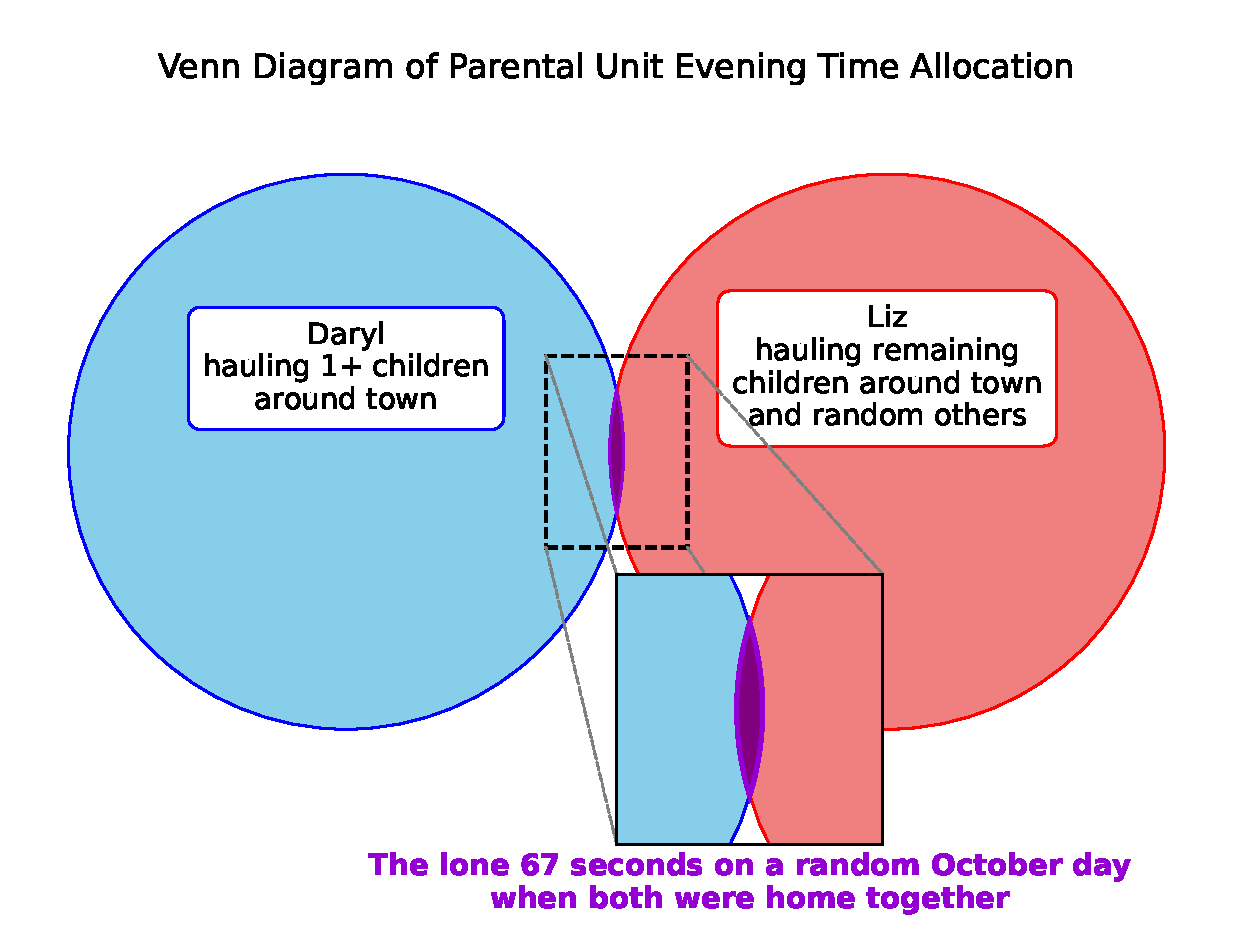
\includegraphics[angle=0]{plots/f1_2025.eps}}
    \caption{Proverbial ships passing in the night.}
\end{figurehere}

Liz remains gainfully employed at Southview Middle School here in Ankeny, attempting to
elevate the science abilities of ${8}^{th}$ grade youth.  She, too, laments Figure~2
and awaits autonomous vehicles or licensable offspring.

\section{Miss Charlotte}

Charlotte is in ${3}^{rd}$ grade.  She plays soccer year-round, loves
science at school, and remains undersized.  She makes up for her lack of
stature with a fiery spirit and fearless nature.  She expertly won an NCAA
men's basketball bracket challenge via the sophisticated methodology of
consistently selecting the superior seed.  Her
soccer team finished second at a tournament in Kansas City.  Her NFL fantasy
football team has a near-perfect losing record for the season.  She dressed up as a
``Flying Squirrel\textsuperscript{™}'' for Halloween (Figure~3)
and continues to wear the costume most days since.

\begin{figurehere}
    \centering   
    \resizebox{.95\columnwidth}{!}{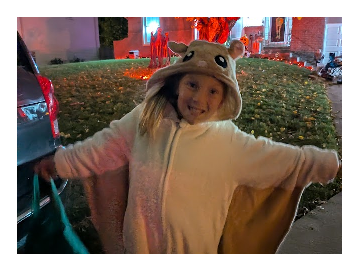
\includegraphics[angle=0]{plots/f3_2025.eps}}
    \caption{Charlotte awaiting glide take-off clearance from FAA.}
\end{figurehere}


\section{Mr Robert}

${6}^{th}$ grader Robert joined \textit{Scouting America} (\textit{a.k.a.} Boy Scouts) this year.
He enjoyed his many camping trips with the troop, arriving home with \keys{0} articles
of dry clothing each time.  He is currently working on another winless season for his
parks-and-rec basketball team.  He joined a robotics club at school and enjoyed a
recent competition.  He also enjoyed an extended weekend helping Grandma's
neighbor harvest corn (Figure~4).

\begin{figurehere}
    \centering
    \resizebox{.95\columnwidth}{!}{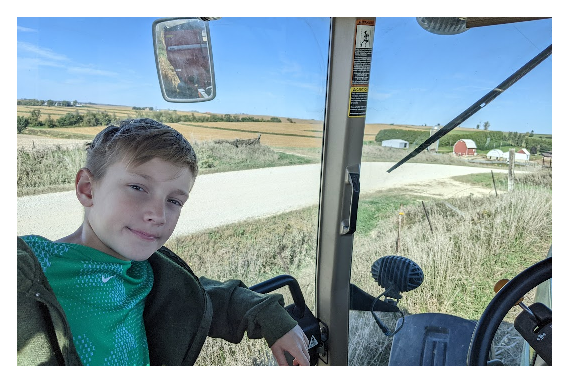
\includegraphics[angle=0]{plots/f4_2025.eps}}
    \caption{Robert with something approximating a smile.}
\end{figurehere}


\section{Miss Maggie}

Maggie is a ${7}^{th}$ grader and mere days away from being an official teenager!
She continues to love school, especially math and science. She just completed the first of two 
band concerts this year. She was also nominated by her band teacher to perform in an 
honor band. She continues to dance and just performed in her fourth rendition of
Tchaikovsky's \textit{Nutcracker}. 
She was Clara this year and loved every second of it. She is also helping out with a 
kindergarten and 1st grade dance class.


\section{Family Vacation}

Our summer family trip was to Rocky Mountain National Park (\ensuremath{\approx} Denver, CO). We first
spent a few days in Colorado Springs and drove up Pikes Peak (\SI{4302}{\meter}),
nearly driving off the side of the mountain six or seven times (Figure~5). 
 Daryl suffered a bout of
\textit{hypoxic syncope} after racing Robert up a small hill. Daryl also got a strange
headache after eating an innocuous brownie from a kindly street vendor
in Boulder, CO.  Liz enjoyed seeing every possible waterfall. The kids enjoyed
our stay at the \textit{Yogi Bear Campground}.

\begin{figurehere}
    \centering   
    \resizebox{.95\columnwidth}{!}{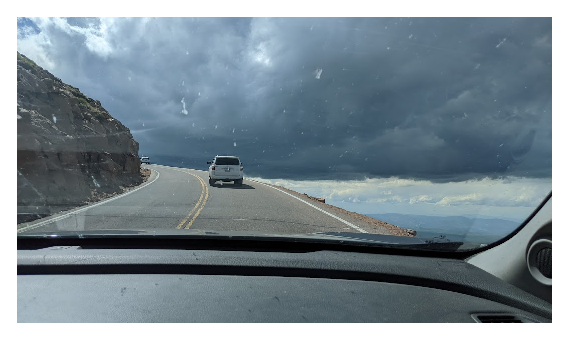
\includegraphics[angle=0]{plots/f5_2025.eps}}
  \caption{Enjoying the view whilst fearing for our lives---nightmare fuel.}
\end{figurehere}

\emph{Acknowledgments} Our family wishes to thank you for the generous 
support, prayers, cards, gifts, and visits you have provided us in the past
year. Additional photos were included this year to self-justify the
outrageous color page charges. Full
\LaTeX\xspace source of this letter can be found on Daryl's GitHub page. 

\section{References}

\refer Herzmann et al. 2021 Christmas Letter.
\refer GitHub. \texttt{https://github.com/akrherz/akrherz}, last viewed on 12 Dec 2025.

\end{multicols}

\end{document}
